\documentclass[12pt]{beamer}
\newenvironment{ConCodigo}[1]
  {\begin{frame}[fragile,environment=ConCodigo]{#1}}
  {\end{frame}}
\graphicspath{{Imagenes/}{../Imagenes/}}
\usepackage[utf8]{inputenc}
\usepackage[spanish]{babel}
\usepackage{hyperref}
\usepackage{etex}
\reserveinserts{28}
\usepackage{amsmath}
\usepackage{amsthm}
\usepackage{mathtools}
\usepackage{multicol}
\usepackage{multirow}
\usepackage{tabulary}
%\usepackage{tabularx}
\usepackage{booktabs}
\usepackage{nccmath}
\usepackage{biblatex}
\usepackage{epstopdf}
\usepackage{graphicx}
\usepackage{siunitx}
\sisetup{scientific-notation=true}
%\usepackage{fontspec}
\usepackage{lmodern}
\usepackage{float}
\usepackage[format=hang, font=footnotesize, labelformat=parens]{caption}
\usepackage[autostyle,spanish=mexican]{csquotes}
\usepackage{standalone}
\usepackage{tikz}
\usepackage[siunitx]{circuitikz}
\usetikzlibrary{arrows,patterns,shapes}
\usetikzlibrary{decorations.markings}
\usetikzlibrary{arrows}
\usepackage{color}
%\usepackage{beton}
%\usepackage{euler}
%\usepackage[T1]{fontenc}
\usepackage[sfdefault]{roboto}  %% Option 'sfdefault' only if the base font of the document is to be sans serif
\usepackage[T1]{fontenc}
\renewcommand*\familydefault{\sfdefault}
\DeclareGraphicsExtensions{.pdf,.png,.jpg}
\usepackage{hyperref}
\renewcommand {\arraystretch}{1.5}
\newcommand{\python}{\texttt{python}}
\usefonttheme[onlymath]{serif}
\setbeamertemplate{navigation symbols}{}
\usetikzlibrary{patterns}
\usetikzlibrary{decorations.markings}
\tikzstyle{every picture}+=[remember picture,baseline]
%\tikzstyle{every node}+=[inner sep=0pt,anchor=base,
%minimum width=2.2cm,align=center,text depth=.15ex,outer sep=1.5pt]
%\tikzstyle{every path}+=[thick, rounded corners]
\setbeamertemplate{caption}[numbered]
\newcommand{\ptm}{\fontfamily{ptm}\selectfont}
%Se usa la plantilla Warsaw modificada con spruce
\mode<presentation>
{
  \usetheme{Warsaw}
  \setbeamertemplate{headline}{}
  \useoutertheme{default}
  \usecolortheme{beaver}
  \setbeamercovered{invisible}
}
\AtBeginSection[]
{
\begin{frame}<beamer>{Contenido}
\normalfont\mdseries
\tableofcontents[currentsection]
\end{frame}
}

\usepackage{epstopdf}
\usepackage{listings}
\lstset{ %
language=Python,                % choose the language of the code
basicstyle=\small,       % the size of the fonts that are used for the code
numbers=left,                   % where to put the line-numbers
numberstyle=\small,      % the size of the fonts that are used for the line-numbers
stepnumber=1,                   % the step between two line-numbers. If it is 1 each line will be numbered
numbersep=5pt,                  % how far the line-numbers are from the code
backgroundcolor=\color{white},  % choose the background color. You must add \usepackage{color}
showspaces=false,               % show spaces adding particular underscores
showstringspaces=false,         % underline spaces within strings
showtabs=false,                 % show tabs within strings adding particular underscores
frame=single,   		% adds a frame around the code
tabsize=2,  		% sets default tabsize to 2 spaces
captionpos=b,   		% sets the caption-position to bottom
breaklines=true,    	% sets automatic line breaking
breakatwhitespace=false,    % sets if automatic breaks should only happen at whitespace
escapeinside={\%},          % if you want to add a comment within your code
stringstyle =\color{magenta},
keywordstyle = \color{blue},
commentstyle = \color{green},
identifierstyle = \color{red}
}
\title{Tema 2 - Operaciones matemáticas básicas}
\subtitle{Técnicas de Interpolación}
\author{M. en C. Gustavo Contreras Mayén}
\begin{document}
\maketitle
\fontsize{14}{14}\selectfont
\spanishdecimal{.}
\begin{frame}{Contenido}
\tableofcontents[pausesections]
\end{frame}
\section{Objetivo}
\begin{frame}
\frametitle{Objetivo General del Tema 2 Operaciones matemáticas básicas}
Al concluir el Tema 2 del curso, el alumno empleará las técnicas más comunes de operaciones matemáticas necesarias para la solución de problemas numéricos apicados en la física.
\\
\medskip
Este tema es una base importante de todo el curso, ya que se establecen las tareas de interpolación, diferenciación e integración numérica y cálculo de raíces, de tal manera que en los temas posteriores, se emplearán las técnicas, en algunos casos, se extenderán de manera específica.
\end{frame}
\section{Introducción.}
\begin{frame}
\frametitle{Iniciamos}
Dados los $n+1$ pares de datos $(x_{i},y_{i})$, con $i=0,1,\ldots,n$, estimar el valor de $y(x)$
\end{frame}
\begin{frame}
Una parte importante en el trabajo del físico es la interpretación de datos experimentales o cálculos teóricos.
\\
\bigskip
Normalmente cuando hacemos mediciones, tenemos un conjunto discreto de puntos que representan nuestro experimento. Para facilitar el trabajo, suponemos que el experimento puede representarse por un par de valores: una \textit{variable independiente x} la cual podemos controlar y una cantidad $y$, que se mide en el punto $x$.
\end{frame}
\begin{frame}
\frametitle{Diferencia entre interpolación y ajuste con curvas}
Hay una diferencia entre interpolación y ajuste de curvas. En la interpolación se \emph{construye una curva a través de los puntos de datos}.
\\
\medskip
El ajuste de curvas se aplica a los datos que contienen una dispersión (ruido), por lo general debida a errores de medición. En este caso, \emph{queremos encontrar una curva suave que se aproxima a los datos en algún sentido}. De tal manera que la curva no toca necesariamente los puntos de datos.
\end{frame}
\begin{frame}[fragile]
\frametitle{Diferencia entre interpolación y ajuste de curvas}

%\begin{tikzpicture}[scale=0.8]
%\draw [->] (0,0) -- (7,0) node [align = left, below] {x};
%\draw [->] (0,0) -- (0,5) node [align = left, above] {y};
%\draw (0.5,0.5)circle (0.1cm);
%\draw (2,1)circle (0.1cm);
%\draw (4.5,2.5)circle (0.1cm);
%\draw (6,4)circle (0.1cm);
%\draw (0,0) .. controls (0.3,0.3) and (0.5,0.5) .. (0.65,0.65)
%			.. controls (0.7,0.7) and (2,1) .. (6.5,4.5);
%\end{tikzpicture}
\begin{figure}
\centering
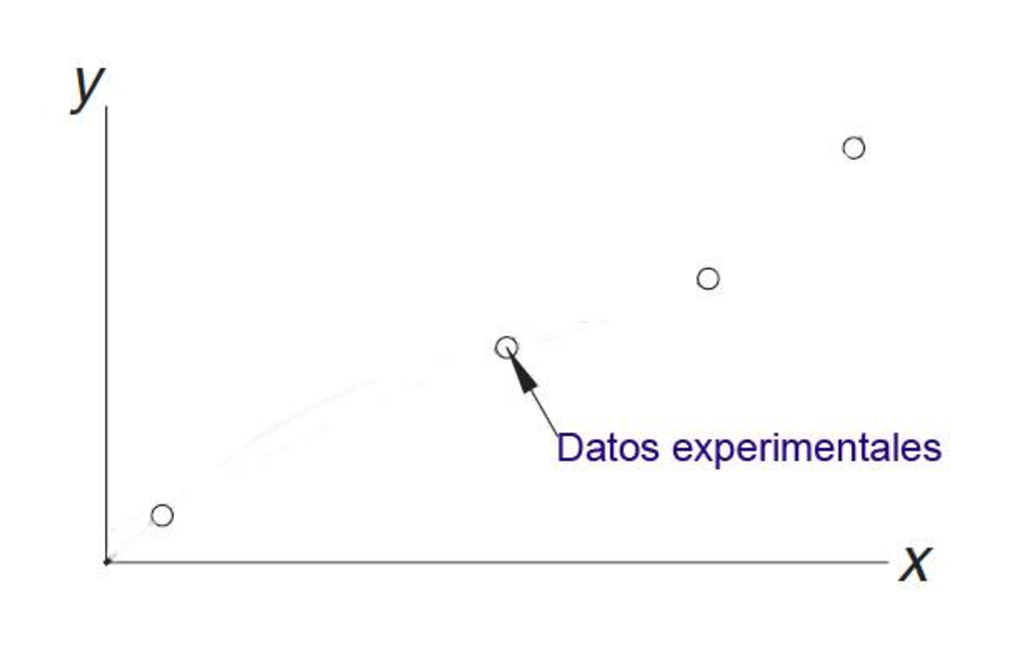
\includegraphics[scale=0.7]{Interpol01.eps}<1>
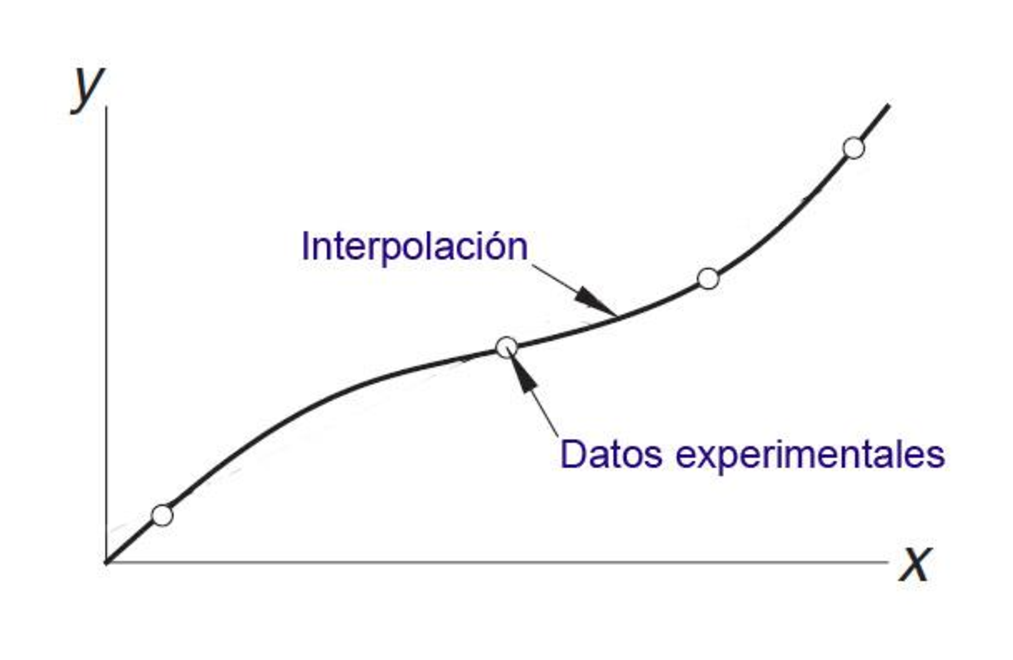
\includegraphics[scale=0.7]{Interpol02.eps}<2>
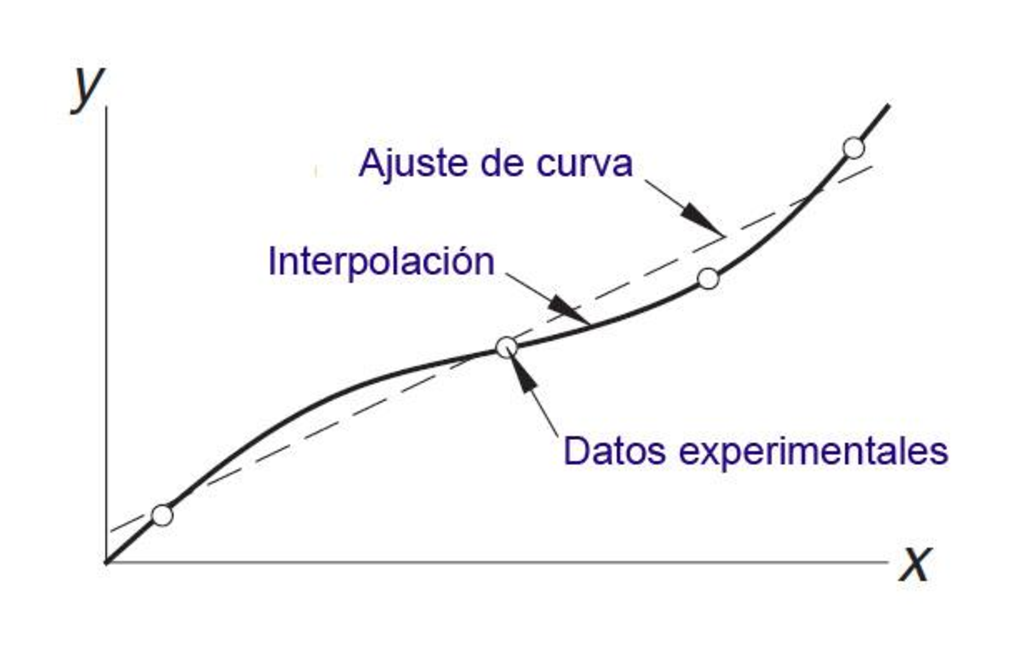
\includegraphics[scale=0.7]{Interpol03.eps}<3>
\end{figure}
\end{frame}
\begin{frame}
Tomemos como ejemplo una fuente radioactiva y un detector, el cual contabiliza el número de decaimientos. Para determinar la vida media de la fuente, debemos de contar los decaimientos $N_{0}$, $N_{1}$, $N_{2}$, $\ldots$, $N_{k}$, en los tiempos $t_{0}$, $t_{1}$, $t_{2}$, $\ldots$, $t_{k}$
\\
\bigskip
En este ejemplo, \textcolor{red}{la variable independiente es $t$}, siendo la forma  apropiada para resolver el problema. Sin embargo, tenemos un conjunto discreto de pares de números $(t_{k},N_{k})$ en el rango de $(t_{0}, t_{k}$)
\end{frame}
\begin{frame}
Con la intención de obtener información del experimento, deberíamos de encontrar una función analítica que nos de el valor de $N$ para cualquier punto arbitrario $t$.
\\
\bigskip
Pero a veces, el tratar de encontrar una función analítica es imposible, o el pensar en utilizar una función conocida, nos podría llevar mucho tiempo para calcularla, más si nuestro interés se basa en una pequeña vecindad de la variable independiente.
\end{frame}
\begin{frame}
\frametitle{Ejemplo}
Supongamos que tenemos una fuente radioactiva de {}$^{241}$Am, una fuente de rayos $\alpha$. Su vida media es $\tau_{\frac{1}{2}}=430$ años.
\\
\bigskip
Obviamente no podríamos determinar su vida media midiéndola, ya que el decaimiento es lento y quizá lo que podríamos hacer es medir cada lunes durante algunos meses. Después de cinco meses (por ejemplo) podríamos detener las mediciones y revisar los datos.
\end{frame}
\begin{frame}
Una pregunta que nos podemos plantear es: ¿cuál fue la actividad el miércoles de la tercera semana de mediciones?  Ya que ese día está dentro del rango de mediciones $(t_{0}, t_{k})$
\end{frame}
\begin{frame}
Lo que podríamos hacer es usar técnicas de \textcolor{blue}{interpolación} para determinar ese valor.  Si lo que queremos, es el caso contrario, conocer la actividad luego de ocho meses posteriores a la última medición, lo que deberíamos de hacer es \textcolor{red}{extrapolar} a ese punto a partir de las mediciones previas.
\end{frame}
\section{Objetivo de la interpolación.}
\begin{frame}
\frametitle{Objetivo de la interpolación.}
La idea central de la interpolación es seleccionar una función $g(x)$ tal que $g(x_{i}) = f_{i}$ para cada dato $i$, es una buena aproximación para cualquier otro dato $x$ entre el conjunto original de datos.
\\
\bigskip
Pero ¿cómo podemos considerar una buena aproximación al conjunto de datos, si no tenemos la función original?
\\
\bigskip
Dado que los puntos ser pueden interpolar por una familia infinita de funciones, para ello debemos de contar con algún criterio o guía para seleccionar una función razonable.
\end{frame}
\begin{frame}
La regla para esos métodos se basa en la \textcolor{red}{suavidad al ajuste} de las funciones de interpolación.
\\
\bigskip
Pero esto no podría funcionar para todo tipo de funciones, consideremos la función:
\\
\medskip
\begin{minipage}{3cm}
\[g(x) = \dfrac{1}{25 x^{2}}\]
\end{minipage}
\hspace{0.5cm}
\begin{minipage}{6cm}
\begin{figure}
	\centering
	 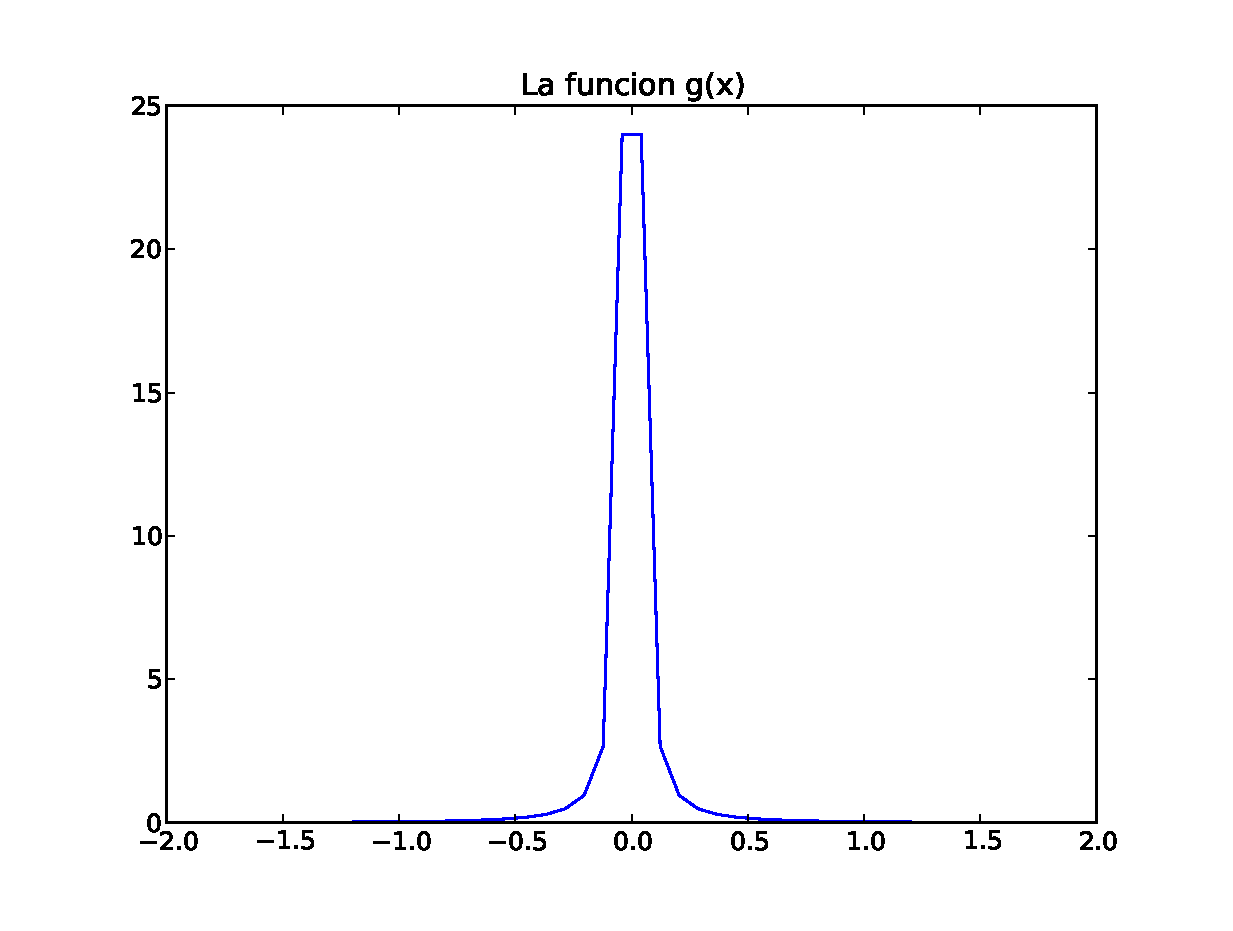
\includegraphics[scale=0.3]{grafica02.eps}  
\end{figure}
\end{minipage}
\end{frame}
\subsection{Consideración previa}
\begin{frame}
\frametitle{Consideración previa}
Antes de entrar de lleno a la revisión de las técnicas de interpolación, es necesario mencionar lo siguiente: dado que contamos con un conjunto finito de puntos, debemos de tener cuidado en el espaciamiento de la variable independiente.
\\
\bigskip
Si los puntos se alejan unos de otros, perderemos información para aquellos valores entre éstos puntos y la predicción de la interpolación ya no será la esperada.
\end{frame}
\begin{frame}
Supongamos que tenemos seis mediciones como se indican en la figura, podemos ver claramente un comportamiento oscilatorio de la función, juzgando por los puntos y de acuerdo a las barras de error, una línea recta es la que probablemente nos ajustaría los puntos.
\begin{figure}
	\centering
	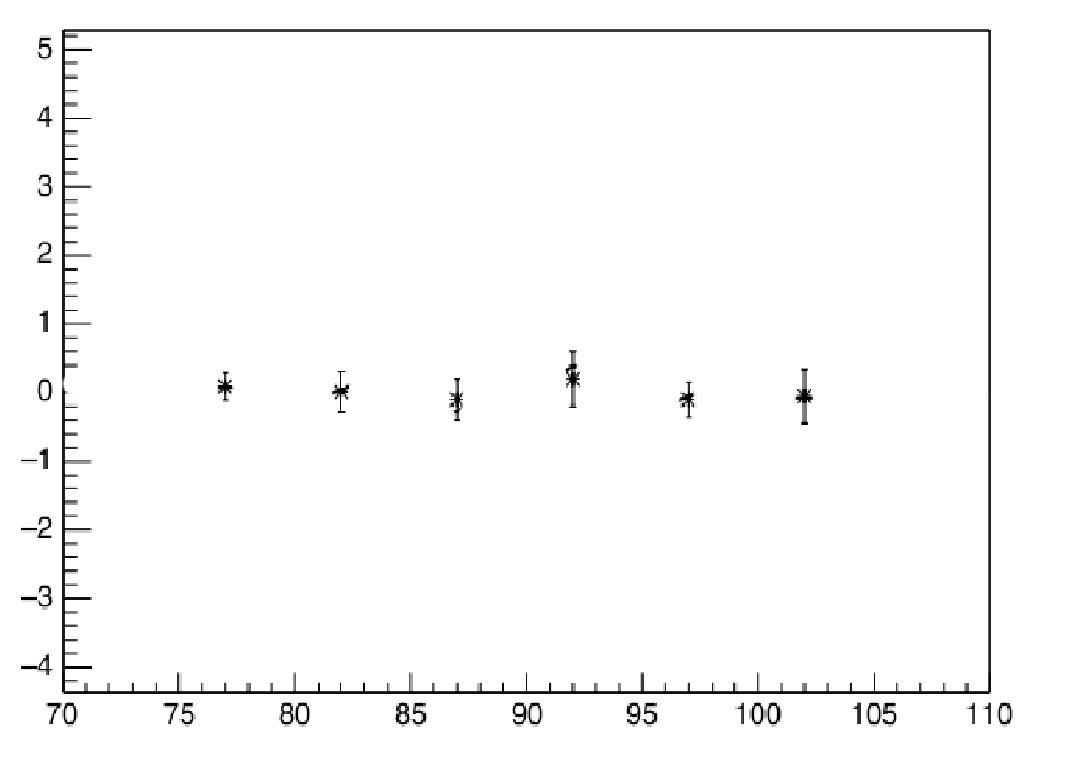
\includegraphics[scale=0.35]{figura01-1.eps} 
\end{figure}
\end{frame}
\begin{frame}
\begin{figure}
	\centering
		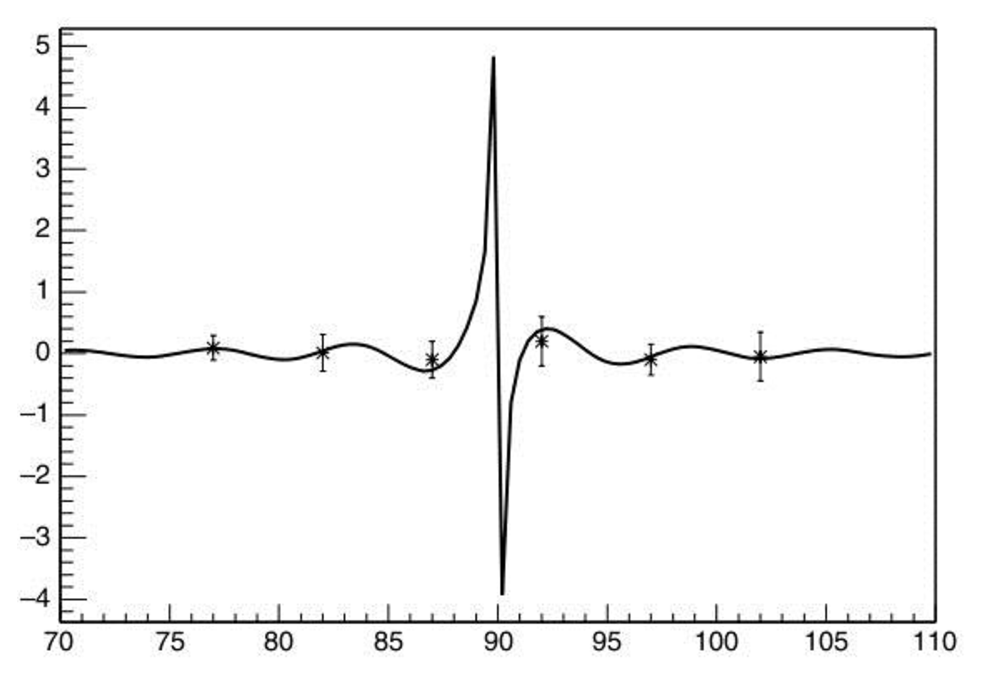
\includegraphics[scale=0.4]{figura02.eps} 
\end{figure}
\end{frame}
\section{Interpolación polinomial}
\subsection{Interpolación de Lagrange}
\begin{frame}
\frametitle{Interpolación de Lagrange}
La técnica más sencilla de interpolación, es usando polinomios. Siempre es posible construir un \emph{único} polinomio de grado $n$ que pasa a través de $n+1$ puntos.
\\
\medskip
Una manera de obtener este polinomio es usando la fórmula de Lagrange

\end{frame}
\begin{frame}
\frametitle{Fórmula de Lagrange}
\[ P_{n}(x) = \sum_{i=0}^{n} y_{i} \mathcal{L}_{i}(x)\]
donde $n$ es el grado del polinomio y
\[ \begin{split}
\mathcal{L}_{i}(x) &= \dfrac{x-x_{0}}{x_{i}-x_{0}} \dfrac{x-x_{1}}{x_{i}-x_{1}} \ldots \dfrac{x-x_{i+1}}{x_{i}-x_{i+1}} \dfrac{x-x_{n}}{x_{i}-x_{n}} \\
 &= \prod_{\substack{j=0 \\ j \neq i}}^{n} \dfrac{x-x_{j}}{x_{i}-x_{j}}, \hspace{0.5cm} i=0,1,\ldots,n
\end{split} \]
se llaman \emph{funciones cardinales}.
\end{frame}
\begin{frame}
\frametitle{Por ejemplo, si $n=1$}
La interpolación es una línea recta: 
\[P_{1}(x) = y_{0}\mathcal{L}_{0}(x) + y_{1} \mathcal{L}_{1}(x) \]
y las funciones cardinales son
\[ \mathcal{L}_{0}(x) = \dfrac{x-x_{1}}{x_{0}-x_{1}} \hspace{1cm} \mathcal{L}_{1}(x) = \dfrac{x-x_{0}}{x_{1}-x_{0}} \]
\end{frame}
\begin{frame}
\frametitle{Con $n=2$}
La interpolación es parabólica:
\[P_{2}(x) = y_{0}\mathcal{L}_{0}(x) + y_{1} \mathcal{L}_{1}(x) + y_{2} \mathcal{L}_{2}(x) \]
y las $\mathcal{L}_{i}(x)$ son:
\begin{eqnarray*}
\mathcal{L}_{0}(x) &=& \dfrac{(x-x_{1})(x-x_{2})}{(x_{0}-x_{1})(x_{0}-x_{2})} \\
\mathcal{L}_{1}(x) &=& \dfrac{(x-x_{0})(x-x_{2})}{(x_{1}-x_{0})(x_{1}-x_{2})} \\
\mathcal{L}_{2}(x) &=& \dfrac{(x-x_{0})(x-x_{1})}{(x_{2}-x_{0})(x_{2}-x_{1})} 
\end{eqnarray*}
\end{frame}
\begin{frame}
\frametitle{Propiedad de las funciones cardinales}
Las funciones cardinales son polinomios de orden $n$ que tiene la propiedad
\[ \mathcal{L}_{i} (x_{j}) = \begin{cases} 0 \hspace{0.1cm} \mbox{si } i \neq j \\ 
1 \hspace{0.1cm} \mbox{si } i = j \end{cases} = \delta_{ij} \]
donde $\delta_{ij}$ es la delta de Kronecker.
\end{frame}
\begin{frame}
Para probar que el polinomio de interpolación pasa por los puntos experimentales, sustituimos $x=x_{j}$ en la definición de $P_{n}(x)$ y usamos el último resultado de $\delta_{ij}$, entonces:
\[ P_{n}(x_{j}) = \sum_{i=0}^{n} y_{i}\mathcal{L}_{i}(x_{j}) = \sum_{i=0}^{n} y_{i} \delta_{ij} = y_{j} \]
\end{frame}
\begin{frame}
Se puede demostrar que el error en el polinomio de interpolación es
\[ f(x) - P_{n}(x) = \dfrac{(x-x_{0})(x-x_{1})\ldots(x-x_{n})}{(n+1)!} f^{(n+1)}(\xi)\]
donde $\xi \in (x_{0},x_{n})$, y éste valor normalmente no se conoce. Debemos de notar que mientras más lejos están los datos de $x$, contribuye a que el error se incremente. 
\end{frame}
\subsubsection{Ejemplo}
\begin{frame}
\frametitle{Ejemplo}
Veamos el cambio de la presión del vapor de {}$^{4}$He como función de la temperatura, de acuerdo a la literatura tenemos que:
\fontsize{12}{12}\selectfont
\begin{center}
\begin{tabular}{c | l@{}}
Temperatura [K] & Presión de vapor [kPa] \\
\hline 2.3 & 6.38512 \\
\hline 2.7 & 13.6218 \\
\hline 2.9 & 18.6760 \\
\hline 3.2 & 28.2599 \\
\hline 3.5 & 40.4082 \\
\hline 3.7 & 49.9945
\end{tabular}
\end{center}
\end{frame}
\begin{frame}
\begin{figure}
	\centering
	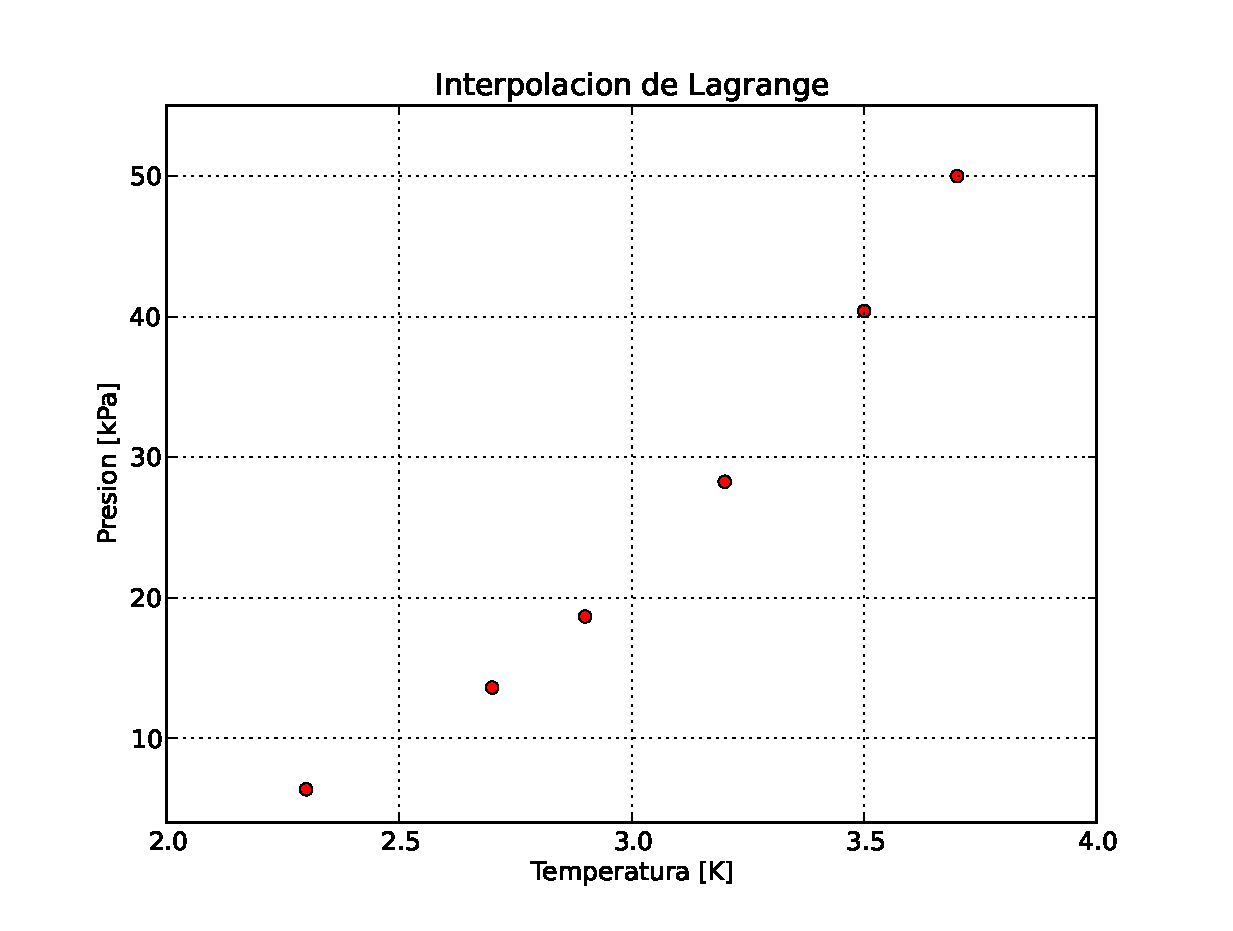
\includegraphics[scale=0.5]{grafica03_1.eps} 
\end{figure}
\end{frame}
\begin{frame}
\begin{figure}
	\centering
	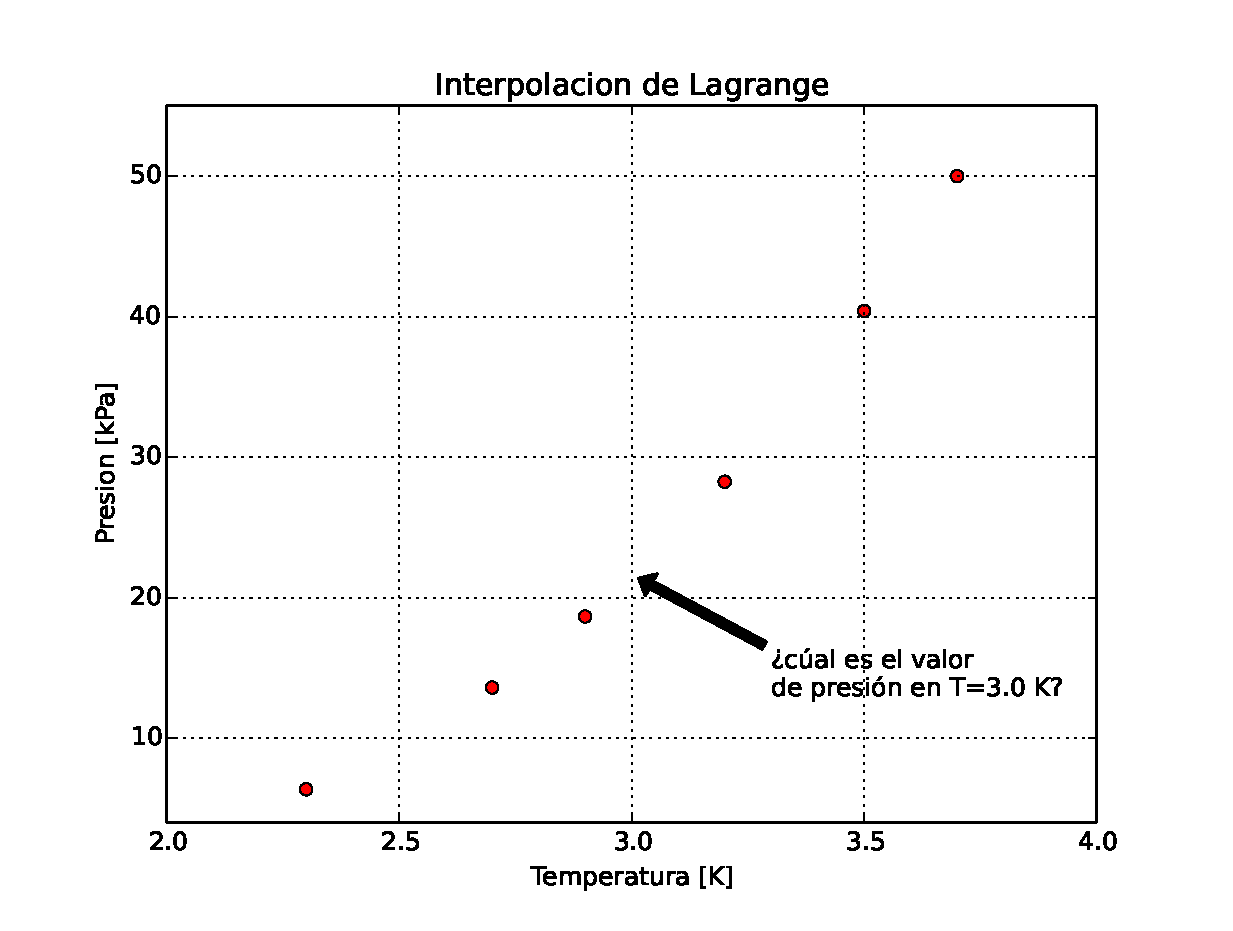
\includegraphics[scale=0.5]{grafica03.eps} 
\end{figure}
\end{frame}
\begin{frame}[fragile]
\frametitle{Solución}
Tomamos lo que ya conocemos para $n=1$
\[P_{1}(x) = y_{0}\mathcal{L}_{0}(x) + y_{1} \mathcal{L}_{1}(x) \]
y las funciones cardinales son
\[ \mathcal{L}_{0}(x) = \dfrac{x-x_{1}}{x_{0}-x_{1}} \hspace{1cm} \mathcal{L}_{1}(x) = \dfrac{x-x_{0}}{x_{1}-x_{0}} \]
En nuestro ejemplo, tenemos que:
\begin{eqnarray*}
(x_{0}, y_{0}) = (2.9, 18.6760) \\
(x_{1}, y_{1}) = (3.2, 28.2599)
\end{eqnarray*}
\visible<2->{Con la interpolación, tenemos que para una temperatura de $3.0$ K, la presión tiene un valor de $21.87$ kPa.}
\end{frame}
\begin{frame}
\frametitle{Interpolación cuadrática}
Con la intención de mejorar nuestro resultado, podemos usar un polinomio de segundo orden, es decir $n=2$
\[P_{2}(x) = y_{0}\mathcal{L}_{0}(x) + y_{1} \mathcal{L}_{1}(x) + y_{2} \mathcal{L}_{2}(x) \]
y las $\mathcal{L}_{i}(x)$ son:
\begin{eqnarray*}
\mathcal{L}_{0}(x) &=& \dfrac{(x-x_{1})(x-x_{2})}{(x_{0}-x_{1})(x_{0}-x_{2})} \\
\mathcal{L}_{1}(x) &=& \dfrac{(x-x_{0})(x-x_{2})}{(x_{1}-x_{0})(x_{1}-x_{2})} \\
\mathcal{L}_{2}(x) &=& \dfrac{(x-x_{0})(x-x_{1})}{(x_{2}-x_{0})(x_{2}-x_{1})} 
\end{eqnarray*}
\end{frame}
\begin{frame}
Usando los valores de la tabla anterior:
\begin{eqnarray*}
(x_{0}, y_{0}) = (2.7, 13.6218) \\
(x_{1}, y_{1}) = (2.9, 18.6760) \\
(x_{2}, y_{2}) = (3.2, 28.2599)
\end{eqnarray*}
\visible<2->{A una temperatura de $3.0$ K, la presión de vapor tiene un valor de 21.671 kPa.}
\\
\bigskip
\visible<3->{El siguiente paso es usar cuatro puntos y construir el polinomio de orden 3.}
\end{frame}
\begin{frame}
\frametitle{Ejercicio}
\begin{minipage}{5cm}
A partir de la siguiente tabla de datos,
\\
\medskip
\begin{center}
\begin{tabular}{c | c}
x & P(x) \\
\hline 1 & 0.671 \\
\hline 2 & 0.620 \\
\hline 3 & 0.567 \\
\hline 4 & 0.512
\end{tabular}
\end{center}
\end{minipage}
\hspace{0.3cm}
\visible<2->{
\begin{minipage}{5cm}
Con el algoritmo de interpolación de Lagrange usando un polinomio de grado 3, estima el valor de $P(x)$ para los siguientes puntos:
\\
\medskip
$x= 1.5,2.5, 3.5,$
\end{minipage}}
\end{frame}
\begin{frame}[fragile]
\begin{lstlisting}[basicstyle=\ttfamily\normalsize, columns=fullflexible]
import numpy as np
n = 3
x0 = np.array([1.5,2.5,3.5])
x = np.array([1., 2., 3., 4.])
f = np.array([0.671, 0.620, 0.567, 0.512])

for k in x0:
    yres = 0
    for i in range(0,n+1):
        z = 1.0
        for j in range(0,n+1):
            if i != j:
                z = z * (k-x[j])/(x[i]-x[j])
        yres = yres + z*f[i]
    print ('El polinomio evaluado en P(',k,') =',  yres)
\end{lstlisting}
\end{frame}
\begin{frame}[fragile]
\frametitle{Solución}
\begin{minipage}{5cm}
\begin{center}
\begin{tabular}{c | l}
x & P(x) \\
\hline 1   & 0.671 \\
\hline 1.5 & 0.64575 \\
\hline 2   & 0.620 \\
\hline 2.5 & 0.59375 \\
\hline 3   & 0.567 \\
\hline 3.5 & 0.53975 \\
\hline 4   & 0.512
\end{tabular}
\end{center}
\end{minipage}
\hspace{0.3cm}
\begin{minipage}{5cm}
\begin{figure}
	\centering
	\includegraphics<1>[scale=0.3]{grafica04.eps}
	\includegraphics<2>[scale=0.3]{grafica04_1.eps}
\end{figure}
\end{minipage}
\end{frame}
\subsection{Ejercicios}
\begin{frame}
\frametitle{Ejercicios}
\begin{enumerate}
\item Ajusta $x \sin(x$) en $[0, \pi/2]$ con un polinomio de interpolación de Lagrange de orden 4, utilizando puntos con igual separación. Calcula el error de cada interpolación en cada incremento de $\pi/16$, muestra una gráfica.
\item Ajusta $\sin(x)$ en $[0, 2\pi]$ con el polinomio de interpolación de Lagrange de orden 4 y 8, utilizando puntos con igual separación (5 y 9 puntos respectivamente). Grafica los polinomios de interpolación junto con $\sin(x)$ y las distribuciones de sus errores.
\end{enumerate}
\end{frame}
\begin{frame}[fragile]
\frametitle{Hints para resolver los ejercicios}
Tomemos en cuenta los siguiente:
\begin{enumerate}[<+->]
\item Hay que dividir el intervalo $[0,\pi/2]$ con cinco espacios.
\item Se evalúa la función $xsin(x)$ en el conjunto de puntos que obtuvimos.
\item Creamos un conjunto de puntos para ajustar con el método de Lagrange.
\item La manera más fácil es con un \texttt{linspace}.
\end{enumerate}
\end{frame}
%\begin{frame}[fragile]
%\frametitle{Obteniendo los datos para el ejercicio}
%\begin{lstlisting}
%n=4
%x0 = linspace(0.,pi/2,20)
%x = linspace(0.,pi/2,5)
%f = funcion(x)
%calculo=[]
%\end{lstlisting}
%\end{frame}
%\begin{frame}[fragile]
%\frametitle{Función f(x)}
%\begin{lstlisting}
%def funcion(x):
%    return x*sin(x)
%\end{lstlisting}
%\end{frame}
%\begin{frame}[fragile]
%\frametitle{Método de Lagrange}
%\begin{lstlisting}
%def metLagrange(n,x0,x):
%    for k in x0:
%        yres = 0
%        for i in range(0,n+1):
%            z = 1.0
%            for j in range(0,n+1):
%                if i != j:
%                    z = z * (k-x[j])/(x[i]-x[j])
%            yres = yres + z*f[i]
%        calculo.append(yres)        
%\end{lstlisting}
%\end{frame}
\begin{frame}
\frametitle{Solución Ejercicio 1}
\begin{figure}
	\centering
	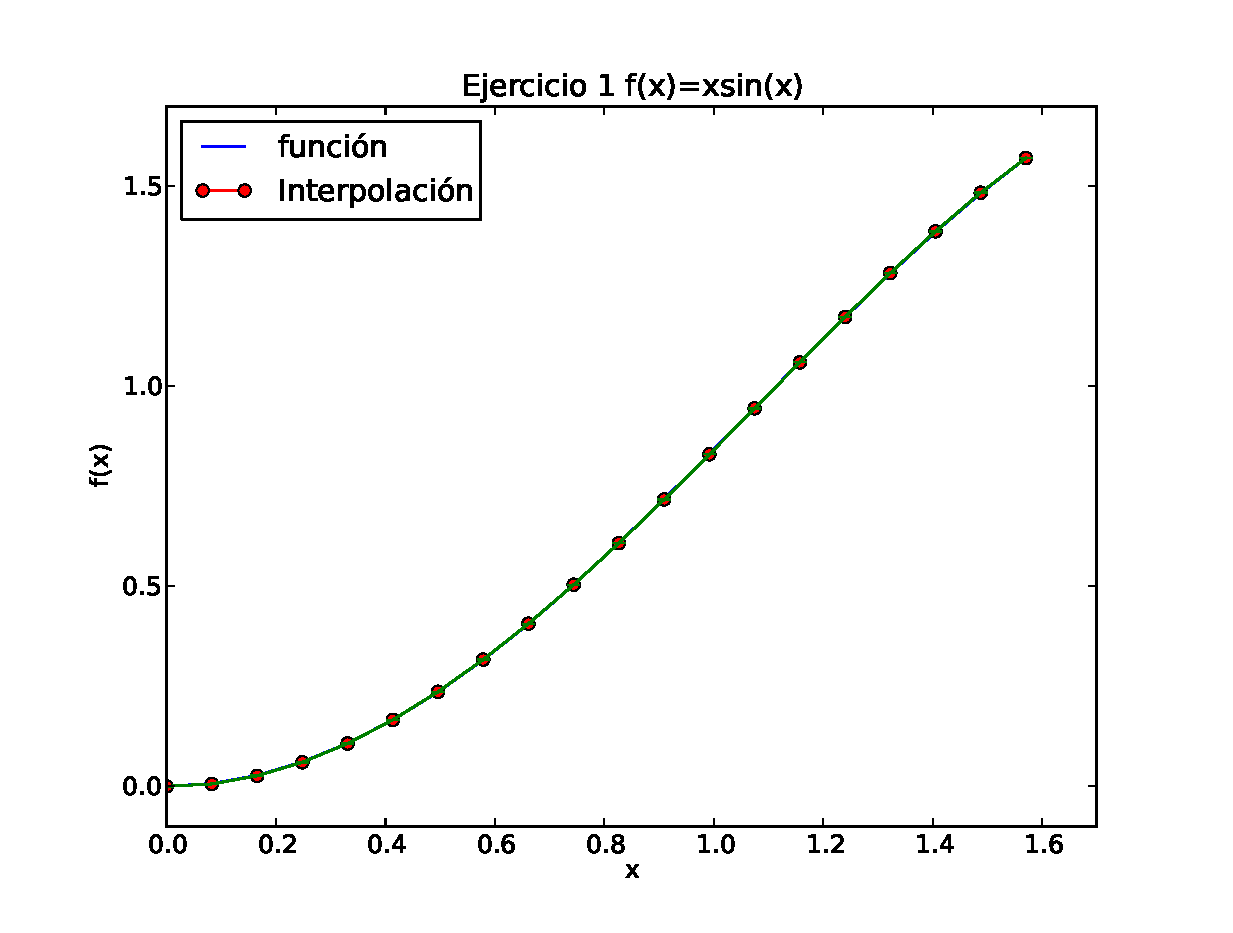
\includegraphics[scale=0.45]{ejercicioTema21_1.eps} 
\end{figure}
\end{frame}
\begin{frame}
\frametitle{Solución Ejercicio 2}
\begin{figure}
	\centering
	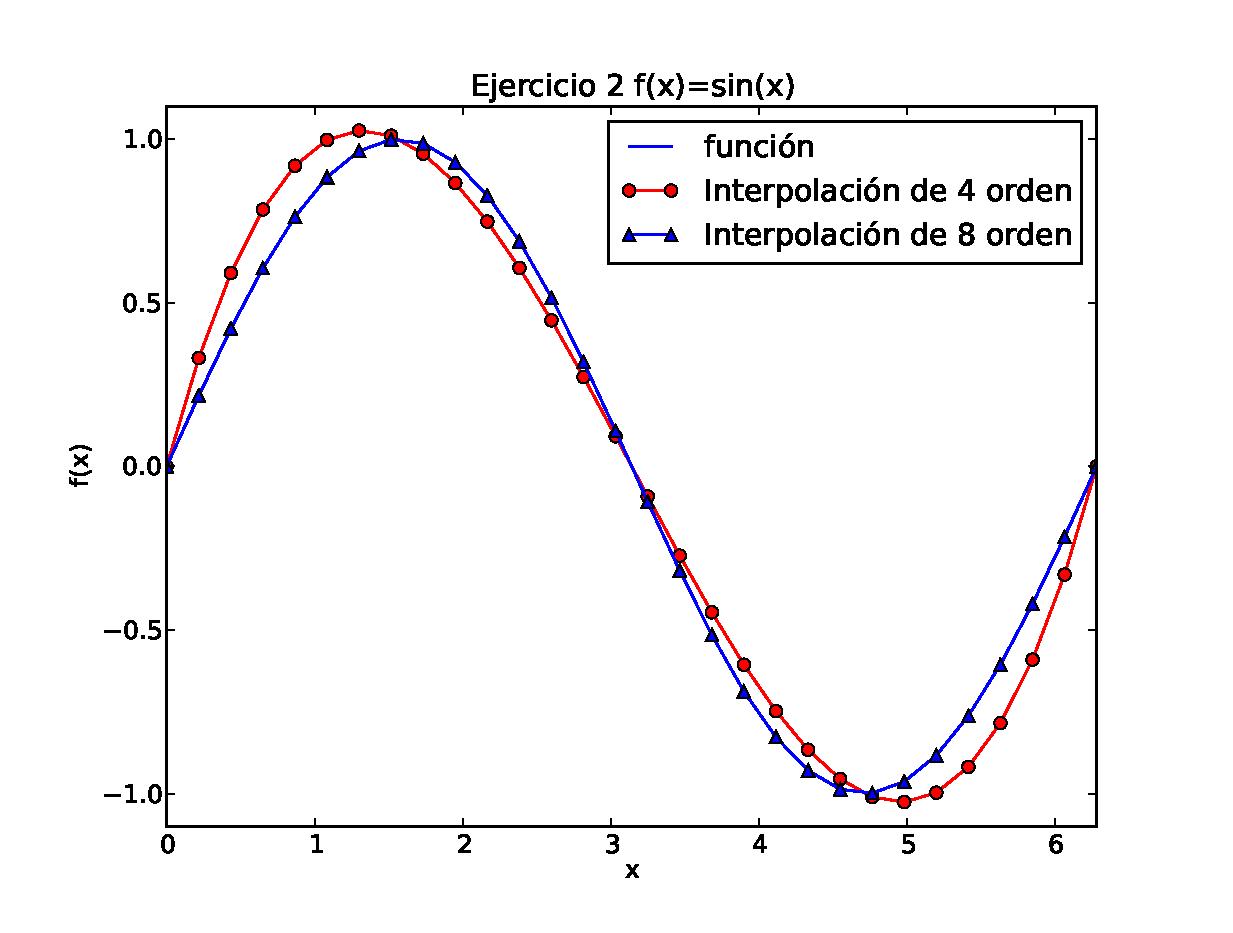
\includegraphics[scale=0.45]{ejercicioTema21_2.eps} 
\end{figure}
\end{frame}
\section{Consideraciones importantes}
\begin{frame}
\frametitle{Consideraciones importantes}
La técnica de interpolación de Lagrange supone que el espaciamiento entre los puntos es la misma, por lo que cuando se presentan puntos que no cumplen ésta condición, la técnica ya no aplicaría.
\\
\bigskip
A continuación se presentan algunas de las desventajas de la primera técnica de interpolación que hemos estudiado.
\end{frame}
\begin{frame}
\frametitle{Desventajas}
\begin{itemize}
\item La cantidad de cálculos necesarios para una interpolación es grande.
\item La interpolación para otro valor de $x$ necesita la misma cantidad de cálculos adicionales, ya que no se pueden utilizar partes de la aplicación previa.
\item Cuando el número de datos tiene que incrementarse o decrementarse, no se pueden utilizar los resultados de los cálculos previos.
\item La evaluación del error no es fácil.
\end{itemize}
\end{frame}
\end{document}